\clearpage
\section{Face-based variables}
\label{sec:face-based}

In all figures in this section, the reader should focus on green parts.
Black ones refer to face-based variables and are kept for reference only.
In the same sense, all occurrences of {\sf n} in text refer to the green 
one (the number of faces), unless stated otherwise.

%%%%%%%%%%%%%%%%%%%%%%%%%
%                       %
%  Sequential Periodic  %
%                       %
%%%%%%%%%%%%%%%%%%%%%%%%%
\subsection{Sequential Periodic}

\subsubsection{Numeration}

%-------------%
%             %
% Face 1.1.1. %
%             %
%-------------%
\begin{figure}[h]
  \centering
  \setlength{\unitlength}{1mm}
  \begin{picture}(105,70)(0,0)
    \thickbox{105}{70}
    \put( 1,0){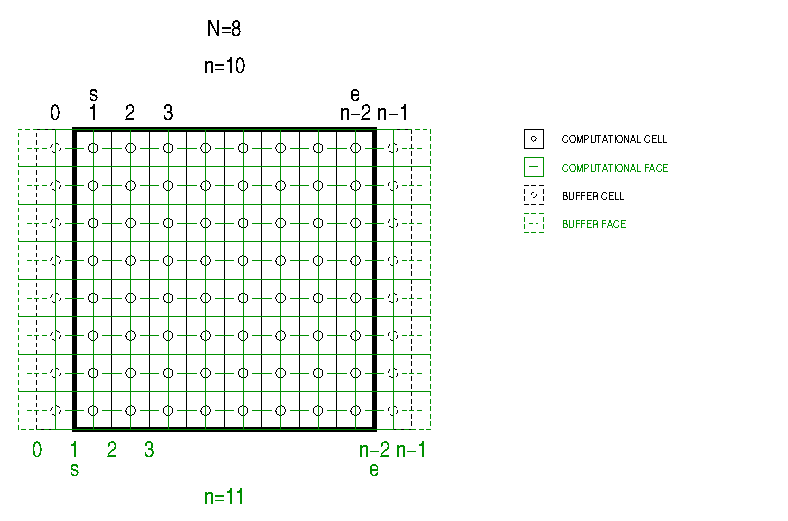
\includegraphics[scale=0.85]{Figures/Face/1periodic_1sequential_1numeration.eps}}
  \end{picture}
  \caption{Numeration of sequential face-based variable with periodic boundary 
           condition.}
  \label{face:111}
\end{figure}

Description of Fig.~\ref{face:111}:
\begin{enumerate}
  \item Number of faces is greater by one than cells 
        (green {\sf n} = black {\sf n + 1}) in the vector direction. 
  \item As for cell-based variables, computational faces are in the range 
        {\sf s} -- {\sf e}, where {\sf s=1} and {\sf e=n-2}.
\end{enumerate}

\subsubsection{Communication}

%-------------%
%             %
% Face 1.1.2. %
%             %
%-------------%
\begin{figure}[h]
  \centering
  \setlength{\unitlength}{1mm}
  \begin{picture}(105,60)(0,0)
    \thickbox{105}{60}
    \put( 1,0){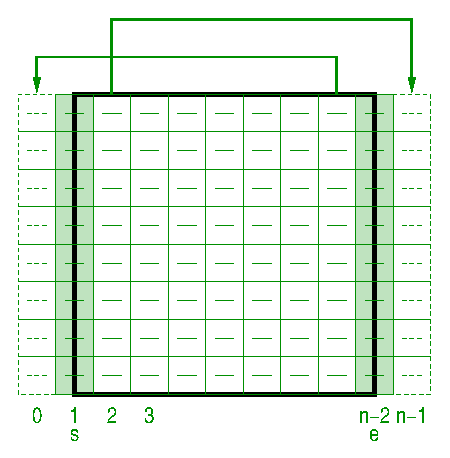
\includegraphics[scale=0.85]{Figures/Face/1periodic_1sequential_2patterns.eps}}
  \end{picture}
  \caption{Communication patterns for sequential face-based variable with 
           periodic boundary condition.}
  \label{face:112}
\end{figure}

Description of Fig.~\ref{face:112}:
\begin{enumerate}
  \item The face value from first ({\sf s}) and last ({\sf e}) are the 
        {\bf same}, but are computed separately. They are {\bf not} exchanged!
  \item Therefore, it is the second computed column ({\sf s+1}) which is sent 
        to the end buffer~({\sf n-1}), while the column before last computed 
        ({\sf e-1}) is sent to the start buffer~({\sf 0}).
  \item The code from {\tt scalar\_exchange.cpp} to achieve this exchange is:
        \begin{verbatim}
         for_jk(j,k) {
           val[e_x+1][j][k] = val[s_x + o_x][j][k];
           val[s_x-1][j][k] = val[e_x - o_x][j][k];
         }
        \end{verbatim}
        Clearly, {\tt o\_x} (offset) is equal to {\bf one} in this case.
\end{enumerate}

%%%%%%%%%%%%%%%%%%%%%%%
%                     %
%  Parallel Periodic  %
%                     %
%%%%%%%%%%%%%%%%%%%%%%%
\subsection{Parallel Periodic}

\subsubsection{Numeration}

%-------------%
%             %
% Face 1.2.1. %
%             %
%-------------%
\begin{figure}[h]
  \centering
  \setlength{\unitlength}{1mm}
  \begin{picture}(105,145)(0,0)
    \thickbox{105}{145}
    \put( 1,0){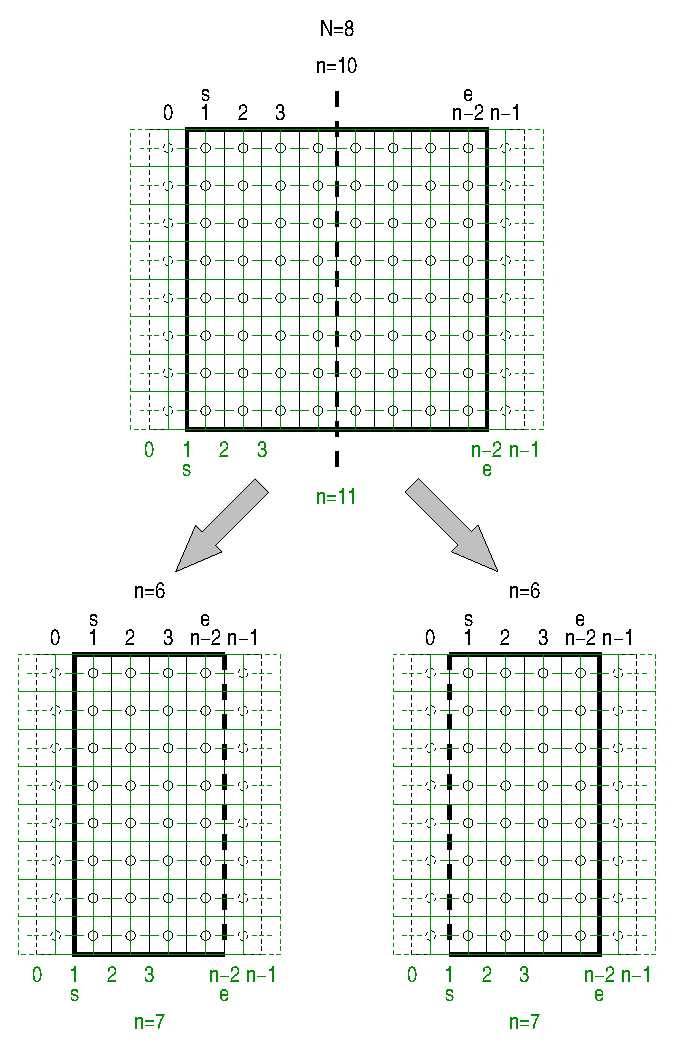
\includegraphics[scale=0.85]{Figures/Face/1periodic_2parallel_1numeration.eps}}
  \end{picture}
  \caption{Numeration of face-based variable with periodic boundary 
           condition for parallel computation.}
  \label{face:121}
\end{figure}

Description of Fig.~\ref{face:121}:
\begin{enumerate}
  \item In case of a parallel run, green {\sf n} is the local number of faces 
        in each processor, including buffers/boundary faces. 
  \item As for the sequential run with periodic boundary conditions, computational 
        faces are in the range {\sf s} -- {\sf e} ({\sf 1} -- {\sf n-2}).
  \item As in sequential case, number of faces is greater than number of cells
        by one: (green {\sf n} = black {\sf n + 1}) in the vector direction.
\end{enumerate}

\subsubsection{Communication}

%-------------%
%             %
% Face 1.2.2. %
%             %
%-------------%
\begin{figure}[h]
  \centering
  \setlength{\unitlength}{1mm}
  \begin{picture}(105,75)(0,0)
    \thickbox{105}{75}
    \put( 1,0){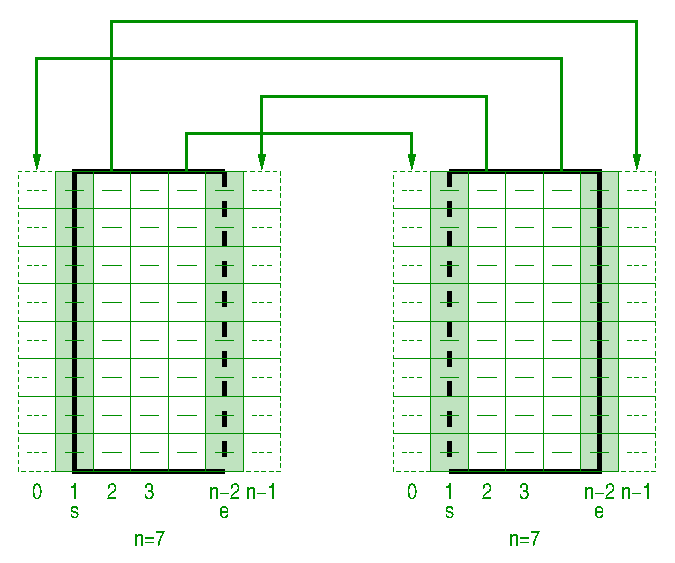
\includegraphics[scale=0.85]{Figures/Face/1periodic_2parallel_2patterns.eps}}
  \end{picture}
  \caption{Communication patterns for parallel face-based variable with 
           periodic boundary condition.}
  \label{face:122}
\end{figure}

Description of Fig.~\ref{face:122}:
\begin{enumerate}
  \item The face value in the last ({\sf e}) column of the left domain is the
        {\bf same} as the face value in the first computed column of the right 
        domain, but they are computed separately. They are {\bf not} exchanged!
  \item Second computed column ({\sf s+1}) is sent to sending buffer at the start
        of the local domain~({\tt sbuff\_s}) and penultimate computed 
        column~({\sf e-1}) is sent to sending buffer at the end of the 
        domain~({\tt sbuff\_e}).
  \item The code from {\tt scalar\_exchange.cpp} to achieve this exchange is the
        same as for cell-based variable:
        \begin{verbatim}
        for_jk(j,k) {
          int l = k*nj()+j;
          sbuff_e[l] = val[e_x - o_x][j][k];   
          sbuff_s[l] = val[s_x + o_x][j][k];  
          rbuff_e[l] = val[e_x +  1 ][j][k];
          rbuff_s[l] = val[s_x -  1 ][j][k];
        }
        \end{verbatim}
        but {\tt o\_x} (offset) is equal to {\bf one} in this case. 
\end{enumerate}

%%%%%%%%%%%%%%%%%%%%%%%%%%%%%
%                           %
%  Sequential Non-periodic  %
%                           %
%%%%%%%%%%%%%%%%%%%%%%%%%%%%%
\clearpage
\subsection{Sequential Non-periodic}

\subsubsection{Numeration}

%-------------%
%             %
% Face 2.1.1. %
%             %
%-------------%
\begin{figure}[h]
  \centering
  \setlength{\unitlength}{1mm}
  \begin{picture}(105,70)(0,0)
    \thickbox{105}{70}
    \put( 1,0){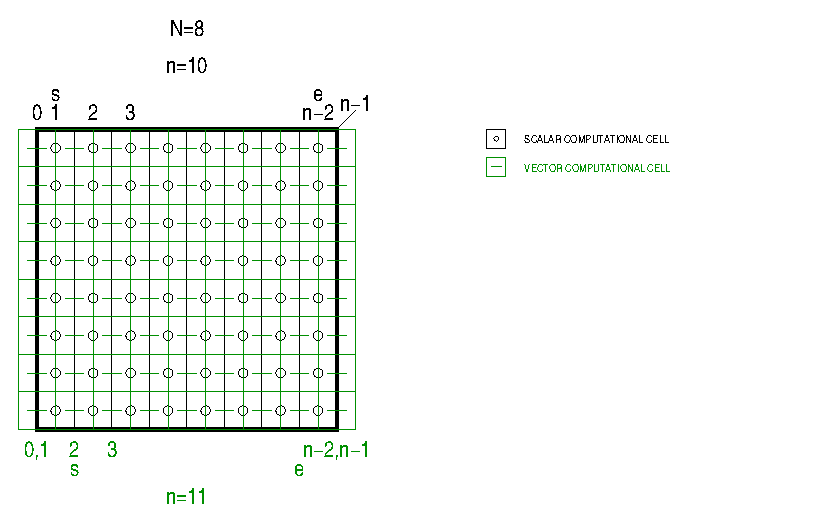
\includegraphics[scale=0.85]{Figures/Face/2non-periodic_1sequential_1numeration.eps}}
  \end{picture}
  \caption{Numeration of sequential face-based variable with non-periodic boundary
           condition.}
  \label{face:211}
\end{figure}

Description of Fig.~\ref{face:211}:
\begin{enumerate}
  \item Boundary faces (column {\sf 0} and {\sf n-1}) coincide with the edge of 
        the computational domain. Since columns {\sf 1} and {\sf n-2} are at the
        domain boundaries as well, columns {\sf 0} and {\sf 1} are at the same place 
        on the left edge of computational domain, while columns {\sf n-2} and 
        {\sf n-1} are at same place on the right edge of the domain.
  \item First computed column ({\sf s}) is no longer {\sf 1} as in the 
        periodic case, but {\sf 2}. Last computed column is not {\sf n-2} as
        in the periodic case, but {\sf n-3}.
\end{enumerate}

%%%%%%%%%%%%%%%%%%%%%%%%%%%
%                         %
%  Parallel Non-periodic  %
%                         %
%%%%%%%%%%%%%%%%%%%%%%%%%%%
\clearpage
\subsection{Parallel Non-periodic}

\subsubsection{Numeration}

%-------------%
%             %
% Face 2.2.1. %
%             %
%-------------%
\begin{figure}[h]
  \centering
  \setlength{\unitlength}{1mm}
  \begin{picture}(105,145)(0,0)
    \thickbox{105}{145}
    \put( 1,0){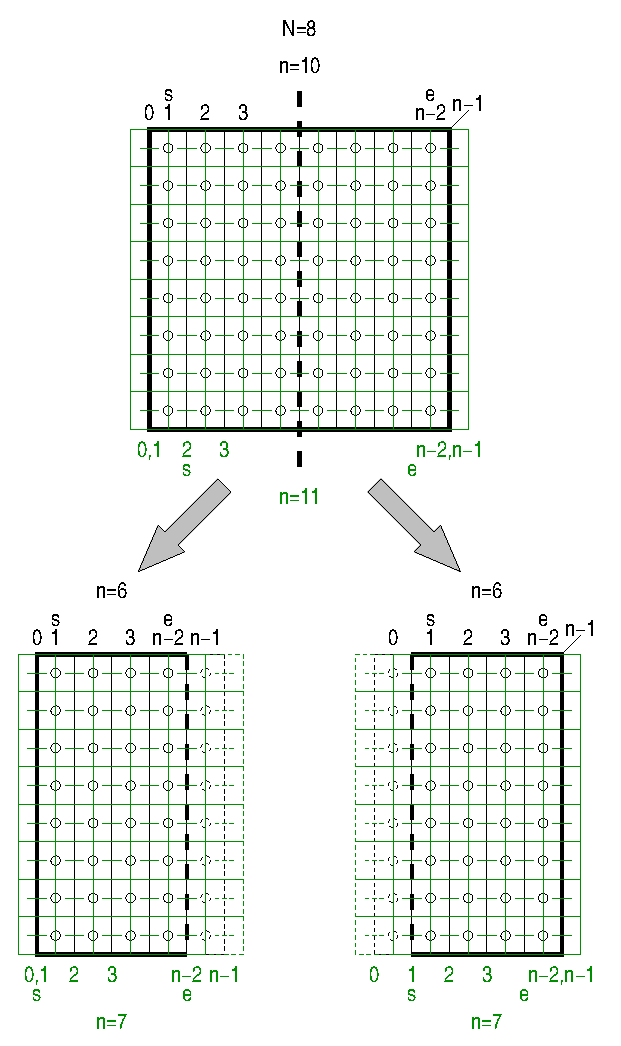
\includegraphics[scale=0.85]{Figures/Face/2non-periodic_2parallel_1numeration.eps}}
  \end{picture}
  \caption{Numeration of sequential face-based variable with non-periodic boundary
           condition.}
  \label{face:221}
\end{figure}

Description of Fig.~\ref{face:221}:
\begin{enumerate}
  \item First computed column ({\sf s}) for the left domain stay {\sf 2}, but 
        last computed column must be adjusted to {\sf n-2}, as if it would be
        for the periodic case.
  \item Last computed column ({\sf e}) for the right domain stays at {\sf n-3},
        but the first ({\sf s}), since at the processor interface, has to change
        to {\sf 1}.
\end{enumerate}

\clearpage
\subsubsection{Communication}

%-------------%
%             %
% Face 2.2.2. %
%             %
%-------------%
\begin{figure}[h]
  \centering
  \setlength{\unitlength}{1mm}
  \begin{picture}(105,65)(0,0)
    \thickbox{105}{65}
    \put( 1,0){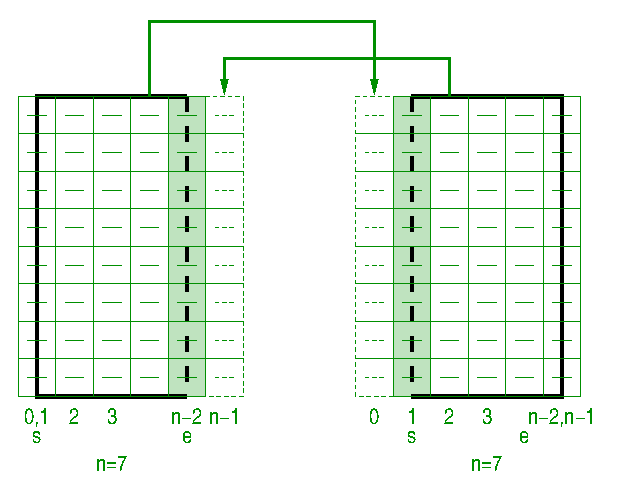
\includegraphics[scale=0.85]{Figures/Face/2non-periodic_2parallel_2patterns.eps}}
  \end{picture}
  \caption{Communication patterns for parallel face-based variable with 
           periodic boundary condition.}
  \label{face:222}
\end{figure}

Description of Fig.~\ref{face:222}:
\begin{enumerate}
  \item Everything is the same as in Fig.~\ref{face:122}, but boundary faces
        (column {\sf 0} in the left and column {\sf n-1} in the right domain) 
        coincide with the edge of the computational domain. Actually, columns
        {\sf 0} and {\sf 1}, as well as {\sf n-2} and {\sf n-1} are at the 
        same place.
\end{enumerate}

%------------------------------------------------------------------------notes-%
\vspace*{5mm} \fbox{ \begin{minipage}[c] {0.97\textwidth} %--------------notes-%
    {\sf Note on other coordinate directions} \\ %-----------------------notes-%

Grid for the face-based variable is staggered only in one direction, while
still cell-centered in the other two, the remaining two directions are
treated in the same way as cell-centered variables. 

  \end{minipage} } %-----------------------------------------------------notes-%
%------------------------------------------------------------------------notes-%
